\subsubsection*{5a) Main Memory}
Processes loaded from disk into memory, logical (virtual) vs. physical address: CPU generates logical addresses, MMU translates to physical (relocation register adds offset). Contiguous allocation: each process occupies a single, continuous memory block.

\textbf{Addr. Binding:} symbolic $\to$ relocatable $\to$ logical $\to$ physical

\textbf{Base/Limit:} base $\leq$ addr $<$ base + limit, trap if violated.

\textbf{Paging:} Divide logical/physical memory into fixed-size pages/frames (power of 2).
Page table maps page \texttt{p} to frame \texttt{f}.
PT in regs (small, fast), PTBR (big, slow, 2 mem acc).
Logical address: (p,d), physical: (f,d).
TLB caches page table entries (solves 2-mem acc).
Protection: read/write/execute, valid/invalid bits.
Shared pages for libraries.
Page table structures: flat (small systems).
hierarchical (multi-level page tables, break big PT $\to$ page-table-walk: several steps needed to access the data frames.
hashed. inverted.

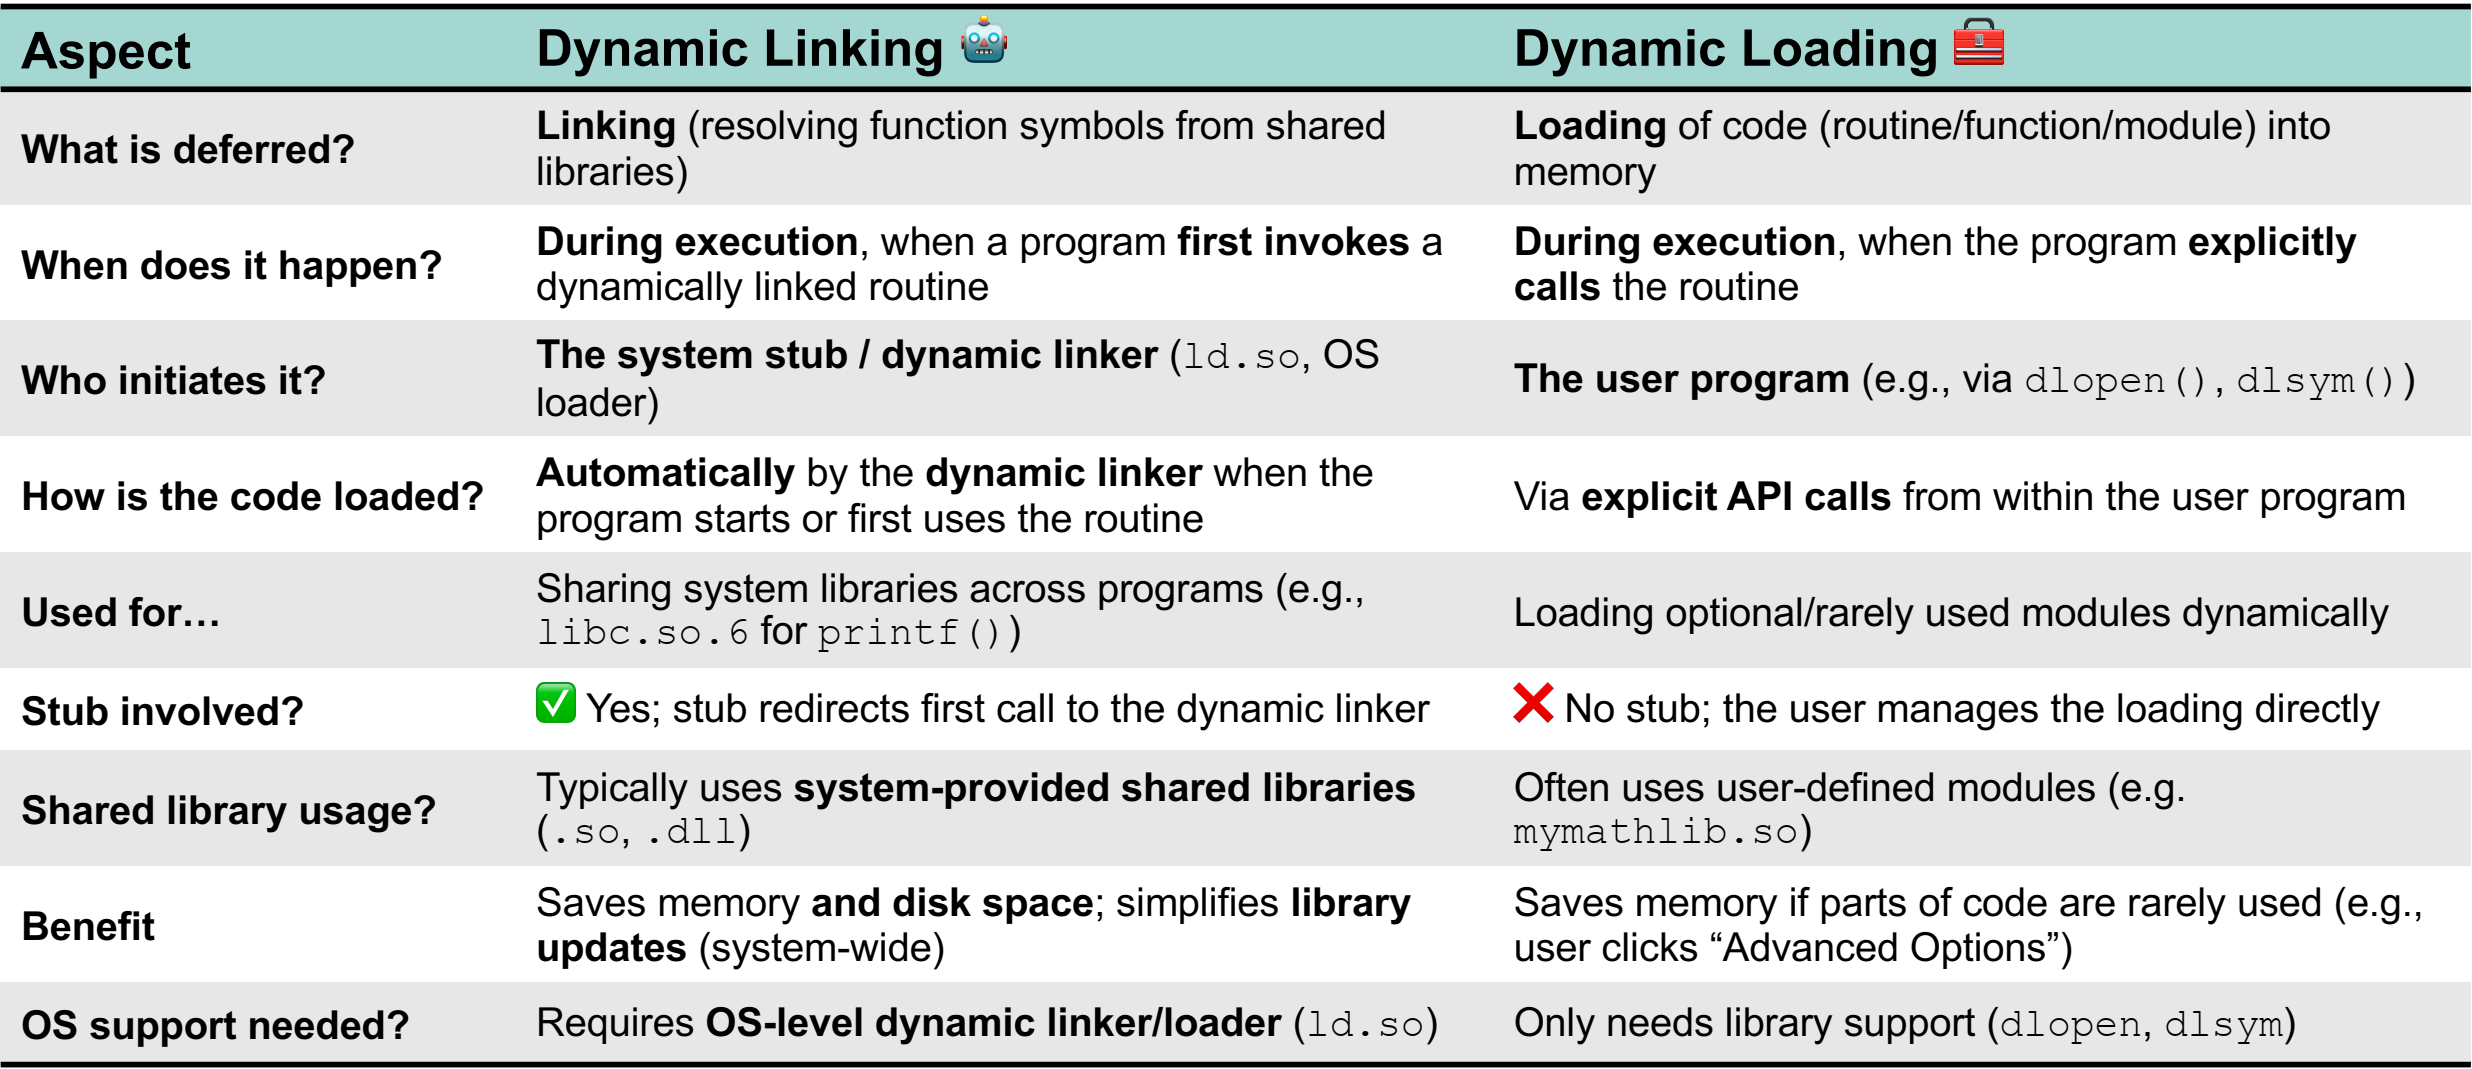
\includegraphics[width=1\linewidth]{images/05a_p21_dyn_link_dyn_load.png}

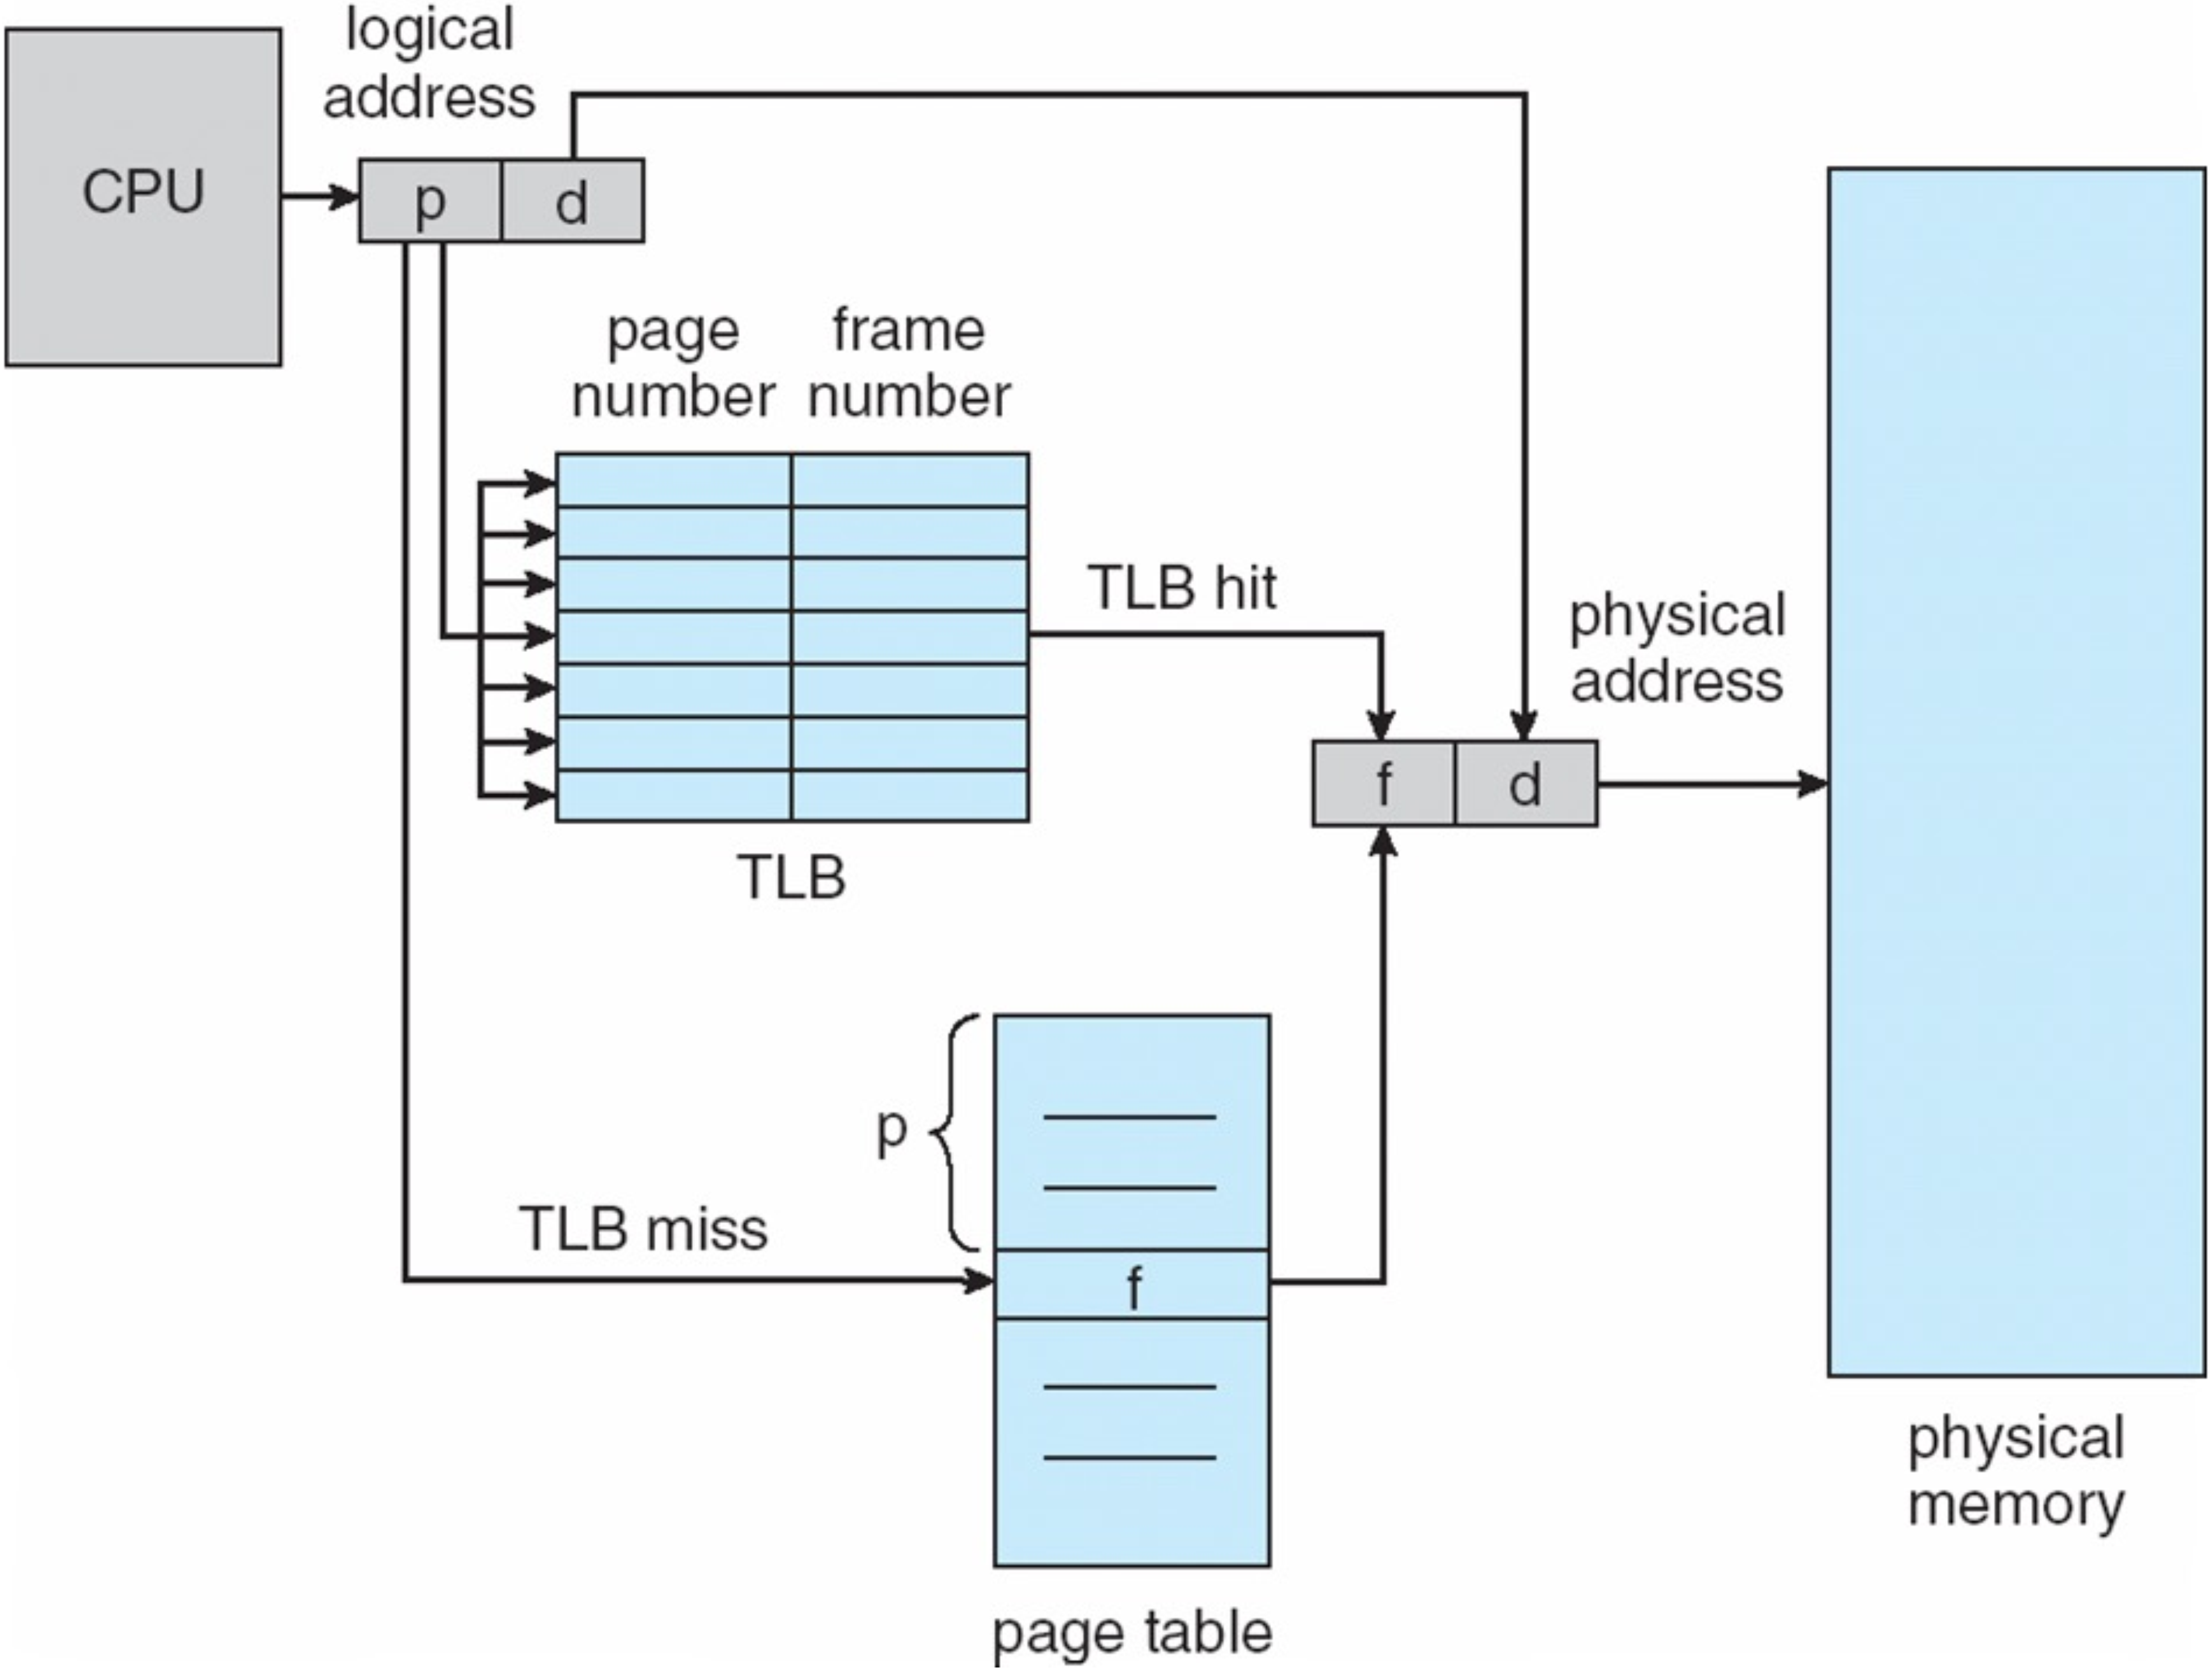
\includegraphics[width=0.95\linewidth]{images/05a_p45_tlb.png}

\textbf{ext. fragmentation}
leftover parts in memory not large enough for any waiting process, because parts not contiguous.
50\% - rule (statistical analysis) for 1st fit: about n/2 blocks are lost to fragmentation $\to$ up to 1/3 of memory may be unusable.

\textbf{Compaction:} reduce ext frag. by moving memory contents to group. Costly, needs dyn. relocation, makes 1 big hole. Static reloc. not possible.

\textbf{int. fragmentation}
physical memory organized and allocated in fixed-size blocks $\to$ wasted space inside the allocated partition if requested size not an exact multiple.

\textbf{Fit Algos:} 1st (fast, ok frag), best (small holes, $\uparrow$ frag), worst (big hole, waste)

\textbf{Swapping:} Move process or pages between RAM and disk (swap space). Supports oversubscription, thrashing risk. Roll-in/out (whole processes), or page-based swapping (demand paging). Swap triggers when memory pressure increases.

\subsubsection*{5b) Virtual Memory}
Allows larger LAS than PAS $\to$ more procs (↑CPU util). Programs partially loaded (demand paging). OS + MMU load pages on-demand, invalid/valid bits track page status. On page fault: trap, find frame, swap page in, update page table, restart. Copy-on-write (COW) on fork: pages shared until written.
Dirty bit: only mod pages → disk.

\textbf{Page replacement:} Find victim frame when no free frame. Algorithms: FIFO (Belady anomaly: ↑frames, ↑faults possible), OPT (not implementable), LRU (hard, approx by Ref bit).

\textbf{Frame allocation:} Equal, proportional (process size/priority), global (all frames), or local (per-process). Global replacement risks trashing (processes competing for frames). Thresholds: low → kernel reclaims; high → suspend reclamation.

\textbf{Trashing:} Excessive page faults due to overcommitment. Fix: add RAM. Locality model: processes use working sets of pages. WS model: \(\Delta\)-window tracks recent page usage; sum of WS sizes \(D\) must fit in RAM. If \(D\) exceeds available frames → suspend processes.

\textbf{Linux:} Global replacement, page lists (active/inactive), kswapd (background page-out daemon). NUMA systems: allocate memory near CPU for efficiency.
